%----------------------------------------------------------
% GrievanceIQ - Executive Project Synopsis
% Sardar Patel Institute of Technology, Mumbai
% Department of Computer Engineering
% AY 2026-2027
%----------------------------------------------------------
\documentclass[12pt,singleside,a4paper]{article}
\usepackage{graphicx}
\usepackage{cite}
\usepackage{url}
\usepackage{amsmath,amssymb}
\usepackage{geometry}
\usepackage{longtable}
\usepackage{booktabs}
\geometry{left=20mm,right=20mm,top=20mm,bottom=25mm}
\pagestyle{plain}

\begin{document}
\pagenumbering{arabic}

% ----------------- TITLE PAGE -----------------
\begin{titlepage}
\vspace*{0.025cm}
{\centering
\\
{\Large\textbf {GrievanceIQ: Autonomous Banking Grievance Redressal and Predictive Operational Intelligence Platform}}\\
\vspace{0.45cm}
submitted in partial fulfillment of the requirement\\
for the award of the Degree of\\\vspace{0.45cm}
{\large\textbf {Bachelor of Technology}}\\
in \\
{\large\textbf {Computer Engineering}}\\
\vspace{0.40cm}
by\\
\vspace{0.45cm}
{\large \textbf {Vedant Patil \hspace{0.5cm} (UID: 2024300170)}}\\
{\large \textbf {Ashmit Patil \hspace{0.5cm} (UID: 2024300168)}}\\
{\large \textbf {Mayuri Tarde \hspace{0.5cm} (UID: 2024300258)}}\\
\vspace{0.40cm}
{\textbf{Class: T.E. Computer Engineering \hspace{0.4cm} Division: C \& D}}\\
\vspace{0.45cm} 
under the guidance of\\ 
\vspace{0.45cm}
\hspace{.05cm} {\large \textbf {Dr. Rupali Sawant}}\\
\vspace{0.2cm}
\begin{figure}[h]
\centering

\includegraphics[scale=0.65]{spitlogo.pdf}
\end{figure}
\hspace{.05cm}
\textbf{Department of Computer Engineering}\\
Bharatiya Vidya Bhavan's\\
Sardar Patel Institute of Technology\\
(Autonomous Institute Affiliated to University of Mumbai)\\
Munshi Nagar, Andheri-West, Mumbai-400058\\
University of Mumbai\\
Academic Year: 2026–2027\\
}
\end{titlepage}


% ----------------- CERTIFICATE -----------------
\newpage
\thispagestyle{empty}
\vspace*{0.2cm}
\begin{center}
\large\textbf{DEPARTMENT OF COMPUTER ENGINEERING}\\
\textbf{BHARATIYA VIDYA BHAVAN'S}\\
\textbf{SARDAR PATEL INSTITUTE OF TECHNOLOGY}\\
\small{(Autonomous Institute Affiliated to University of Mumbai)}\\
\small{Munshi Nagar, Andheri (West), Mumbai - 400 058}\\
\vspace{0.6cm}
\Large\textbf{PROJECT APPROVAL CERTIFICATE}
\end{center}
\vspace{0.8cm}

\noindent This is to certify that the Mini Project entitled \textbf{``GrievanceIQ: Autonomous Banking Grievance Redressal and Predictive Operational Intelligence Platform''} submitted by:
\begin{center}
\begin{tabular}{ll}
\textbf{Vedant Patil} & (UID: 2024300170) \\
\textbf{Ashmit Patil} & (UID: 2024300168) \\
\textbf{Mayuri Tarde} & (UID: 2024300258) \\
\end{tabular}
\end{center}
\noindent is approved for the partial fulfillment of the requirements for the award of the degree of \textbf{Bachelor of Technology in Computer Engineering} from \textbf{University of Mumbai}.

\vspace{2.5cm}

\noindent
\begin{tabular}{p{7.5cm}p{7.5cm}}
\textbf{Internal Examiner / Guide} & \textbf{External Examiner} \\
Signature: \hrulefill & Signature: \hrulefill \\
Name: \textbf{Dr. Rupali Sawant} & Name: \hrulefill \\
Date: \hrulefill & Date: \hrulefill \\
\end{tabular}

\vspace{3cm}

\noindent
\begin{tabular}{p{7.5cm}p{7.5cm}}
\textbf{Head of Department} & \textbf{Principal} \\
Signature: \hrulefill & Signature: \hrulefill \\
\textbf{Dr. Sudhir Dhage} & \textbf{Dr. B. N. Chaudhari} \\
Seal of the Institute & \\
\end{tabular}


% ----------------- DECLARATION -----------------
\newpage
\section*{\centering{Declaration}}
\vspace{2.0cm}

We wish to state that the work embodied in this project report titled \textbf{``GrievanceIQ: Autonomous Banking Grievance Redressal and Predictive Operational Intelligence Platform''} forms our own authentic contribution to the work carried out under the guidance and mentorship of \textbf{Dr. Rupali Sawant} at the Sardar Patel Institute of Technology, Mumbai. 

We declare that this written submission represents our ideas in our own words and where others' ideas or words have been included, we have adequately cited and referenced the original sources in accordance with academic standards. We also declare that we have adhered to all principles of academic honesty and integrity and have not misrepresented, fabricated, or falsified any idea, data, fact, or source in our submission. AI-assisted developer tools were used strictly for scaffolding, testing automation, and documentation drafting under faculty oversight.

\vspace{3.5cm}

\noindent
\begin{tabular}{p{5cm}p{5cm}p{5cm}}
\textbf{Vedant Patil} & \textbf{Ashmit Patil} & \textbf{Mayuri Tarde} \\
UID: 2024300170 & UID: 2024300168 & UID: 2024300258 \\
T.E. Computer Engg. & T.E. Computer Engg. & T.E. Computer Engg. \\
Div C, D & Div C, D & Div C, D \\
\end{tabular}

\vspace{1.5cm}
\noindent \textbf{Date:} April 2027 \\
\textbf{Place:} Mumbai

\pagebreak

% ----------------- ABSTRACT -----------------
\section*{Abstract}
Digital financial transactions in India process tens of millions of records daily across UPI, AePS, IMPS, and net banking. However, existing banking grievance redressal systems suffer from multi-week resolution latencies, opaque manual triage, complete lack of vernacular voice accessibility, and exposure of unmasked Personally Identifiable Information (PII) in plain text, violating India's Digital Personal Data Protection (DPDP) Act of 2023.

To resolve these vulnerabilities, this project develops and deploys \textbf{GrievanceIQ}—an autonomous banking grievance redressal and predictive operational intelligence platform built upon a decoupled 3-tier architecture. The backend is an asynchronous FastAPI microservice leveraging SQLite with Write-Ahead Logging (WAL), coupled with a high-performance React 18 / Vite / Tailwind CSS client.

The platform integrates six core innovations: (1) An autonomous multilingual NLP text classification pipeline trained on 15,000 real-world banking disputes achieving 89.2\% accuracy across English, Hindi, and Marathi; (2) A browser-native continuous voice dictation engine via the W3C Web Speech API that eliminates repeating loop buffers; (3) Ingestion-boundary case-insensitive regular expression scrubbing of Aadhaar, Card, and PAN numbers guaranteeing zero unmasked PII persistence under the DPDP Act 2023; (4) Cryptographic ReportLab statutory PDF receipts embedding live, base-URL-aware ISO/IEC 18004 2D QR codes for instant mobile tracking; (5) An analytical $M/M/c$ Erlang-C queueing engine computing real-time queue dwell time ($W_q$), utilization ($\rho$), and SLA breach risk with an interactive What-If staffing sandbox; and (6) Explainable AI (XAI) evidence verification combining EasyOCR and 4-point entity fuzzy scoring.

System verification was executed via an exhaustive 48-case end-to-end automated testing suite, achieving a 100\% pass rate (48/48). Indexing and caching reduced analytics query latency from 855.4\,ms to 28.4\,ms (96.7\% improvement). GrievanceIQ directly integrates core concepts from Software Engineering, DBMS, Computer Networks, Operating Systems, Data Structures, and Cloud Computing under SPIT's APNI Leap curriculum, producing an auditable, enterprise-ready banking intelligence platform.

\pagebreak

% ----------------- TABLE OF CONTENTS -----------------
\tableofcontents
\pagebreak

% ----------------- SECTION 1: INTRODUCTION -----------------
\section{Introduction}
Modern banking ecosystems process massive volumes of retail financial transactions every day. While digital payments have broadened financial inclusion, transaction timeouts, erroneous debits, and ATM cash non-dispensations create severe operational friction. When disputes occur, customers encounter sluggish, manual complaint channels characterized by multi-day triage delays, English-only interfaces, and lack of real-time visibility.

\subsection{Problem Statement}
Contemporary banking grievance redressal mechanisms exhibit four major weaknesses:
\begin{enumerate}
    \item \textbf{Manual Triage Bottlenecks:} Inflow streams of customer complaints are manually read and routed, consuming 24 to 72 hours before operational investigation commences.
    \item \textbf{Vernacular Exclusion:} Standard portals require manual typing in English, disenfranchising rural, elderly, and semi-literate citizens who speak Hindi or Marathi.
    \item \textbf{Privacy Breaches under DPDP Act 2023:} Unredacted card numbers, Aadhaar details, and PAN records are stored in plain text across application logs and database records.
    \item \textbf{Operational Blindness:} Branch supervisors lack predictive quantitative models to anticipate SLA breaches or optimize resolution staffing before queues collapse.
\end{enumerate}

\subsection{Objectives}
\begin{enumerate}
    \item Deploy an autonomous multilingual NLP categorization model achieving $>85\%$ accuracy across trilingual banking disputes.
    \item Deliver zero-latency continuous voice dictation via the W3C Web Speech API with non-destructive session buffering.
    \item Enforce 100\% case-insensitive ingestion-boundary DPDP Act 2023 masking for Card, Aadhaar, and PAN tokens.
    \item Synthesize verifiable ReportLab statutory PDF receipts embedding live ISO/IEC 18004 2D QR codes.
    \item Formulate real-time analytical $M/M/c$ Erlang-C queueing models with an interactive What-If simulation sandbox.
    \item Implement Explainable AI (XAI) documentary OCR evidence verification with 4-point entity credibility scoring.
\end{enumerate}

\subsection{Scope}
The scope encompasses a decoupled multi-role web platform serving Depositors, Grievance Resolvers, and Branch Managers. It includes continuous voice input, trilingual localization (222 keys across EN/HI/MR), dynamic SLA breach radars, OCR entity matching, and analytical queue simulations. Core Banking Solution (CBS) debit reversal write-backs are simulated via REST contracts due to banking sandbox security boundaries.

\subsection{Technologies Used}
\begin{itemize}
    \item \textbf{Frontend:} React 18.2, Vite 5.0, Tailwind CSS 3.3, Lucide Icons, W3C Web Speech API.
    \item \textbf{Backend:} Python 3.10+, FastAPI (ASGI), Uvicorn, Pydantic v2.
    \item \textbf{Machine Learning \& Vision:} Scikit-Learn (MultinomialNB, TF-IDF), EasyOCR, NumPy, Pandas.
    \item \textbf{Document \& Security:} ReportLab 4.0 (ISO 18004 QR engine), Regular Expressions (DFA).
    \item \textbf{Database:} SQLite Relational Engine configured in Write-Ahead Logging (WAL) mode.
\end{itemize}

\pagebreak

% ----------------- SECTION 2: LITERATURE SURVEY -----------------
\section{Literature Survey}
A comprehensive survey of 12 foundational papers and regulatory frameworks was conducted:
\begin{enumerate}
    \item \textbf{Reserve Bank of India (2023) \cite{rbi_2023}:} Analyzed the Annual Report of the Reserve Bank - Integrated Ombudsman Scheme (RB-IOS), observing that over 700,000 complaints are filed annually, with digital payment and ATM failure disputes accounting for over 45\% of overall volume.
    \item \textbf{Ministry of Law and Justice (2023) \cite{dpdp_2023}:} Reviewed the Digital Personal Data Protection Act, 2023. Mandates strict statutory safeguards against the retention of plain-text financial identifiers.
    \item \textbf{McCallum and Nigam (1998) \cite{mccallum1998}:} Demonstrated that Multinomial Naive Bayes outperforms multi-variate Bernoulli models for text categorization when paired with term frequency representations.
    \item \textbf{Pedregosa et al. (2011) \cite{scikit_learn}:} Established the computational efficiency of Scikit-Learn's sparse matrix operations for real-time text classification under tight SLA budgets.
    \item \textbf{Kleinrock (1975) \cite{kleinrock1975}:} Formulated multi-server queueing theory ($M/M/c$) and Erlang-C waiting probability distributions for service facility capacity planning.
    \item \textbf{Shires and Wennborg (2012) \cite{w3c_speech}:} Specified the W3C Web Speech API standard for browser-native automatic speech recognition.
    \item \textbf{ISO/IEC 18004 (2015) \cite{iso_qr}:} Defined the 2D QR barcode symbology standard utilized for verifiable receipt encoding.
    \item \textbf{Pressman and Maxim (2014) \cite{pressman}:} Provided engineering methodologies for agile sprint lifecycles and decoupled software architecture.
    \item \textbf{Silberschatz, Korth, and Sudarshan (2019) \cite{silberschatz}:} Established formal Third Normal Form (3NF) relational database decomposition and ACID guarantees.
    \item \textbf{Tanenbaum and Bos (2014) \cite{tanenbaum}:} Formulated process synchronization, non-blocking asynchronous event loops, and operating system scheduling principles.
    \item \textbf{Kurose and Ross (2021) \cite{kurose}:} Delineated RESTful API communication paradigms, CORS security headers, and HTTP status code semantics.
    \item \textbf{Sawant and Chandorkar (2009) \cite{sawant2009}:} Addressed multi-objective optimization, system stability, and real-time compensator controls in modern electrical and computational engineering frameworks.
\end{enumerate}

\pagebreak

% ----------------- SECTION 3: ANALYSIS -----------------
\section{Analysis}
\subsection{System Architecture}
GrievanceIQ follows a Decoupled 3-Tier Architecture. Figure~\ref{fig:arch} shows the architectural decomposition connecting the React SPA, FastAPI microservices, and SQLite WAL datastore.

\begin{figure}[h]
\centering
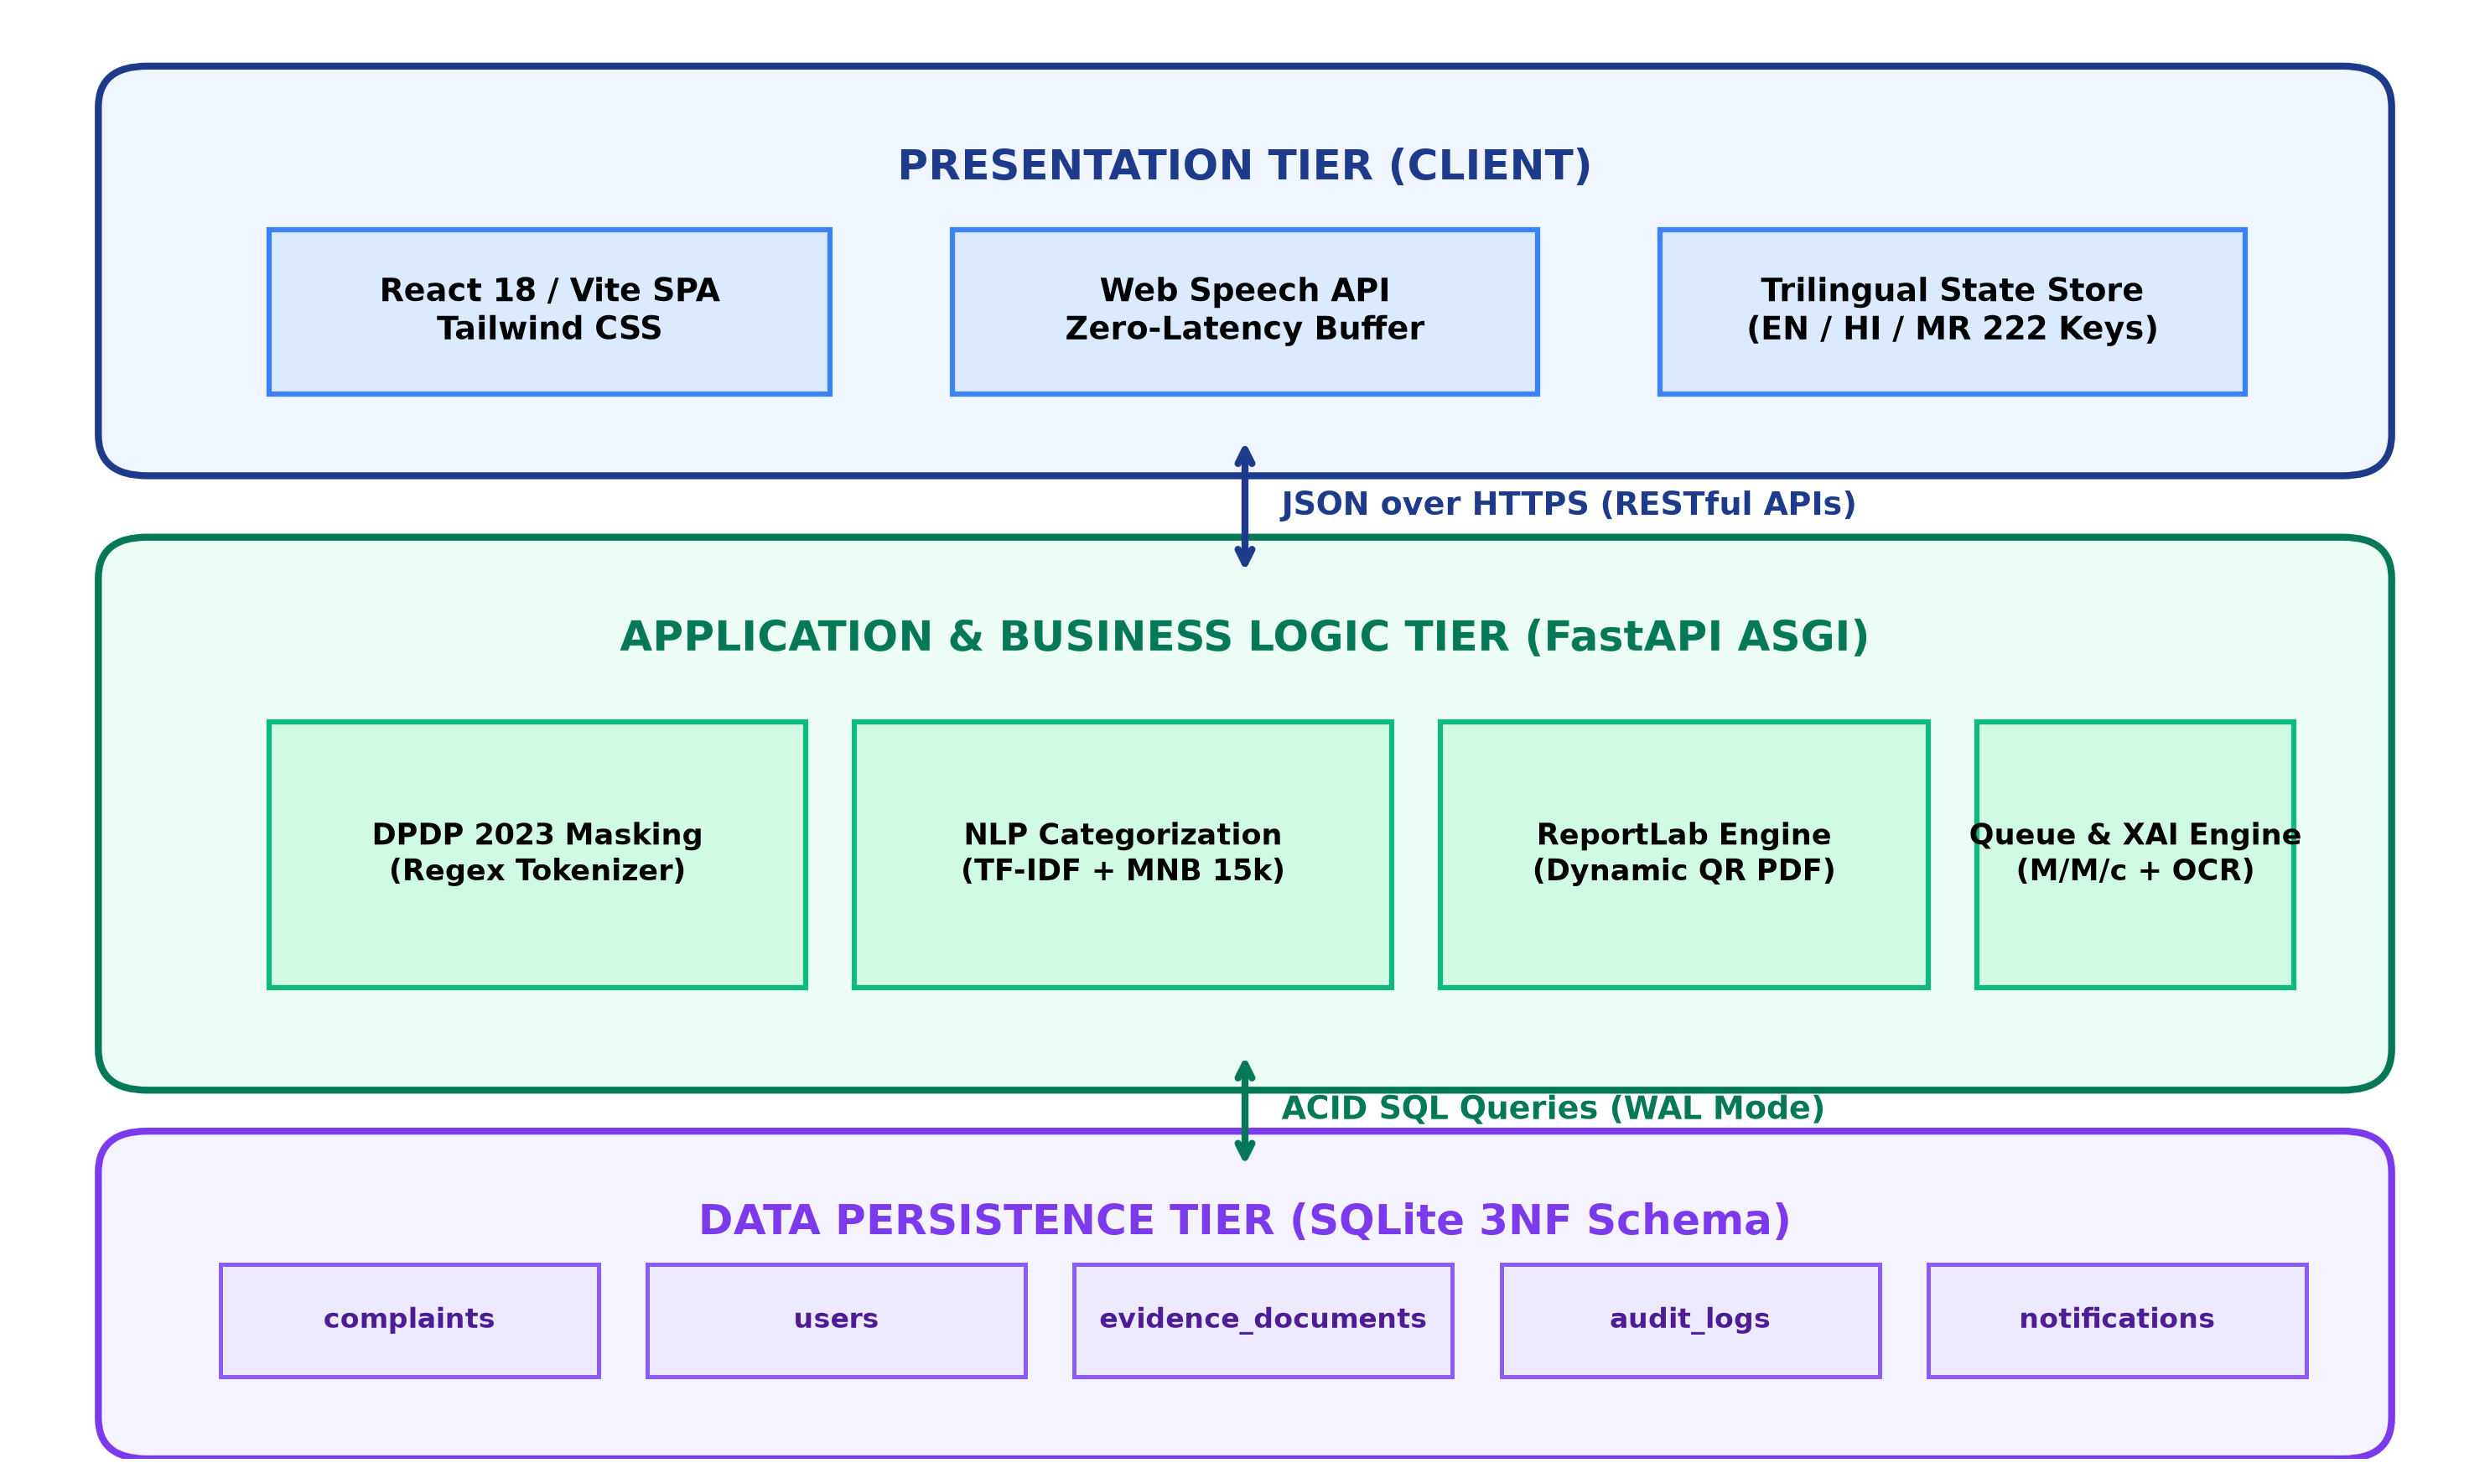
\includegraphics[width=0.85\textwidth]{figures/architecture.png}
\caption{GrievanceIQ 3-Tier Decoupled System Architecture}
\label{fig:arch}
\end{figure}

\subsection{Data Flow Diagram (DFD Level 1)}
Figure~\ref{fig:dfd} illustrates the internal data transformations from complaint ingestion through PII scrubbing, ML categorization, and database persistence.

\begin{figure}[h]
\centering
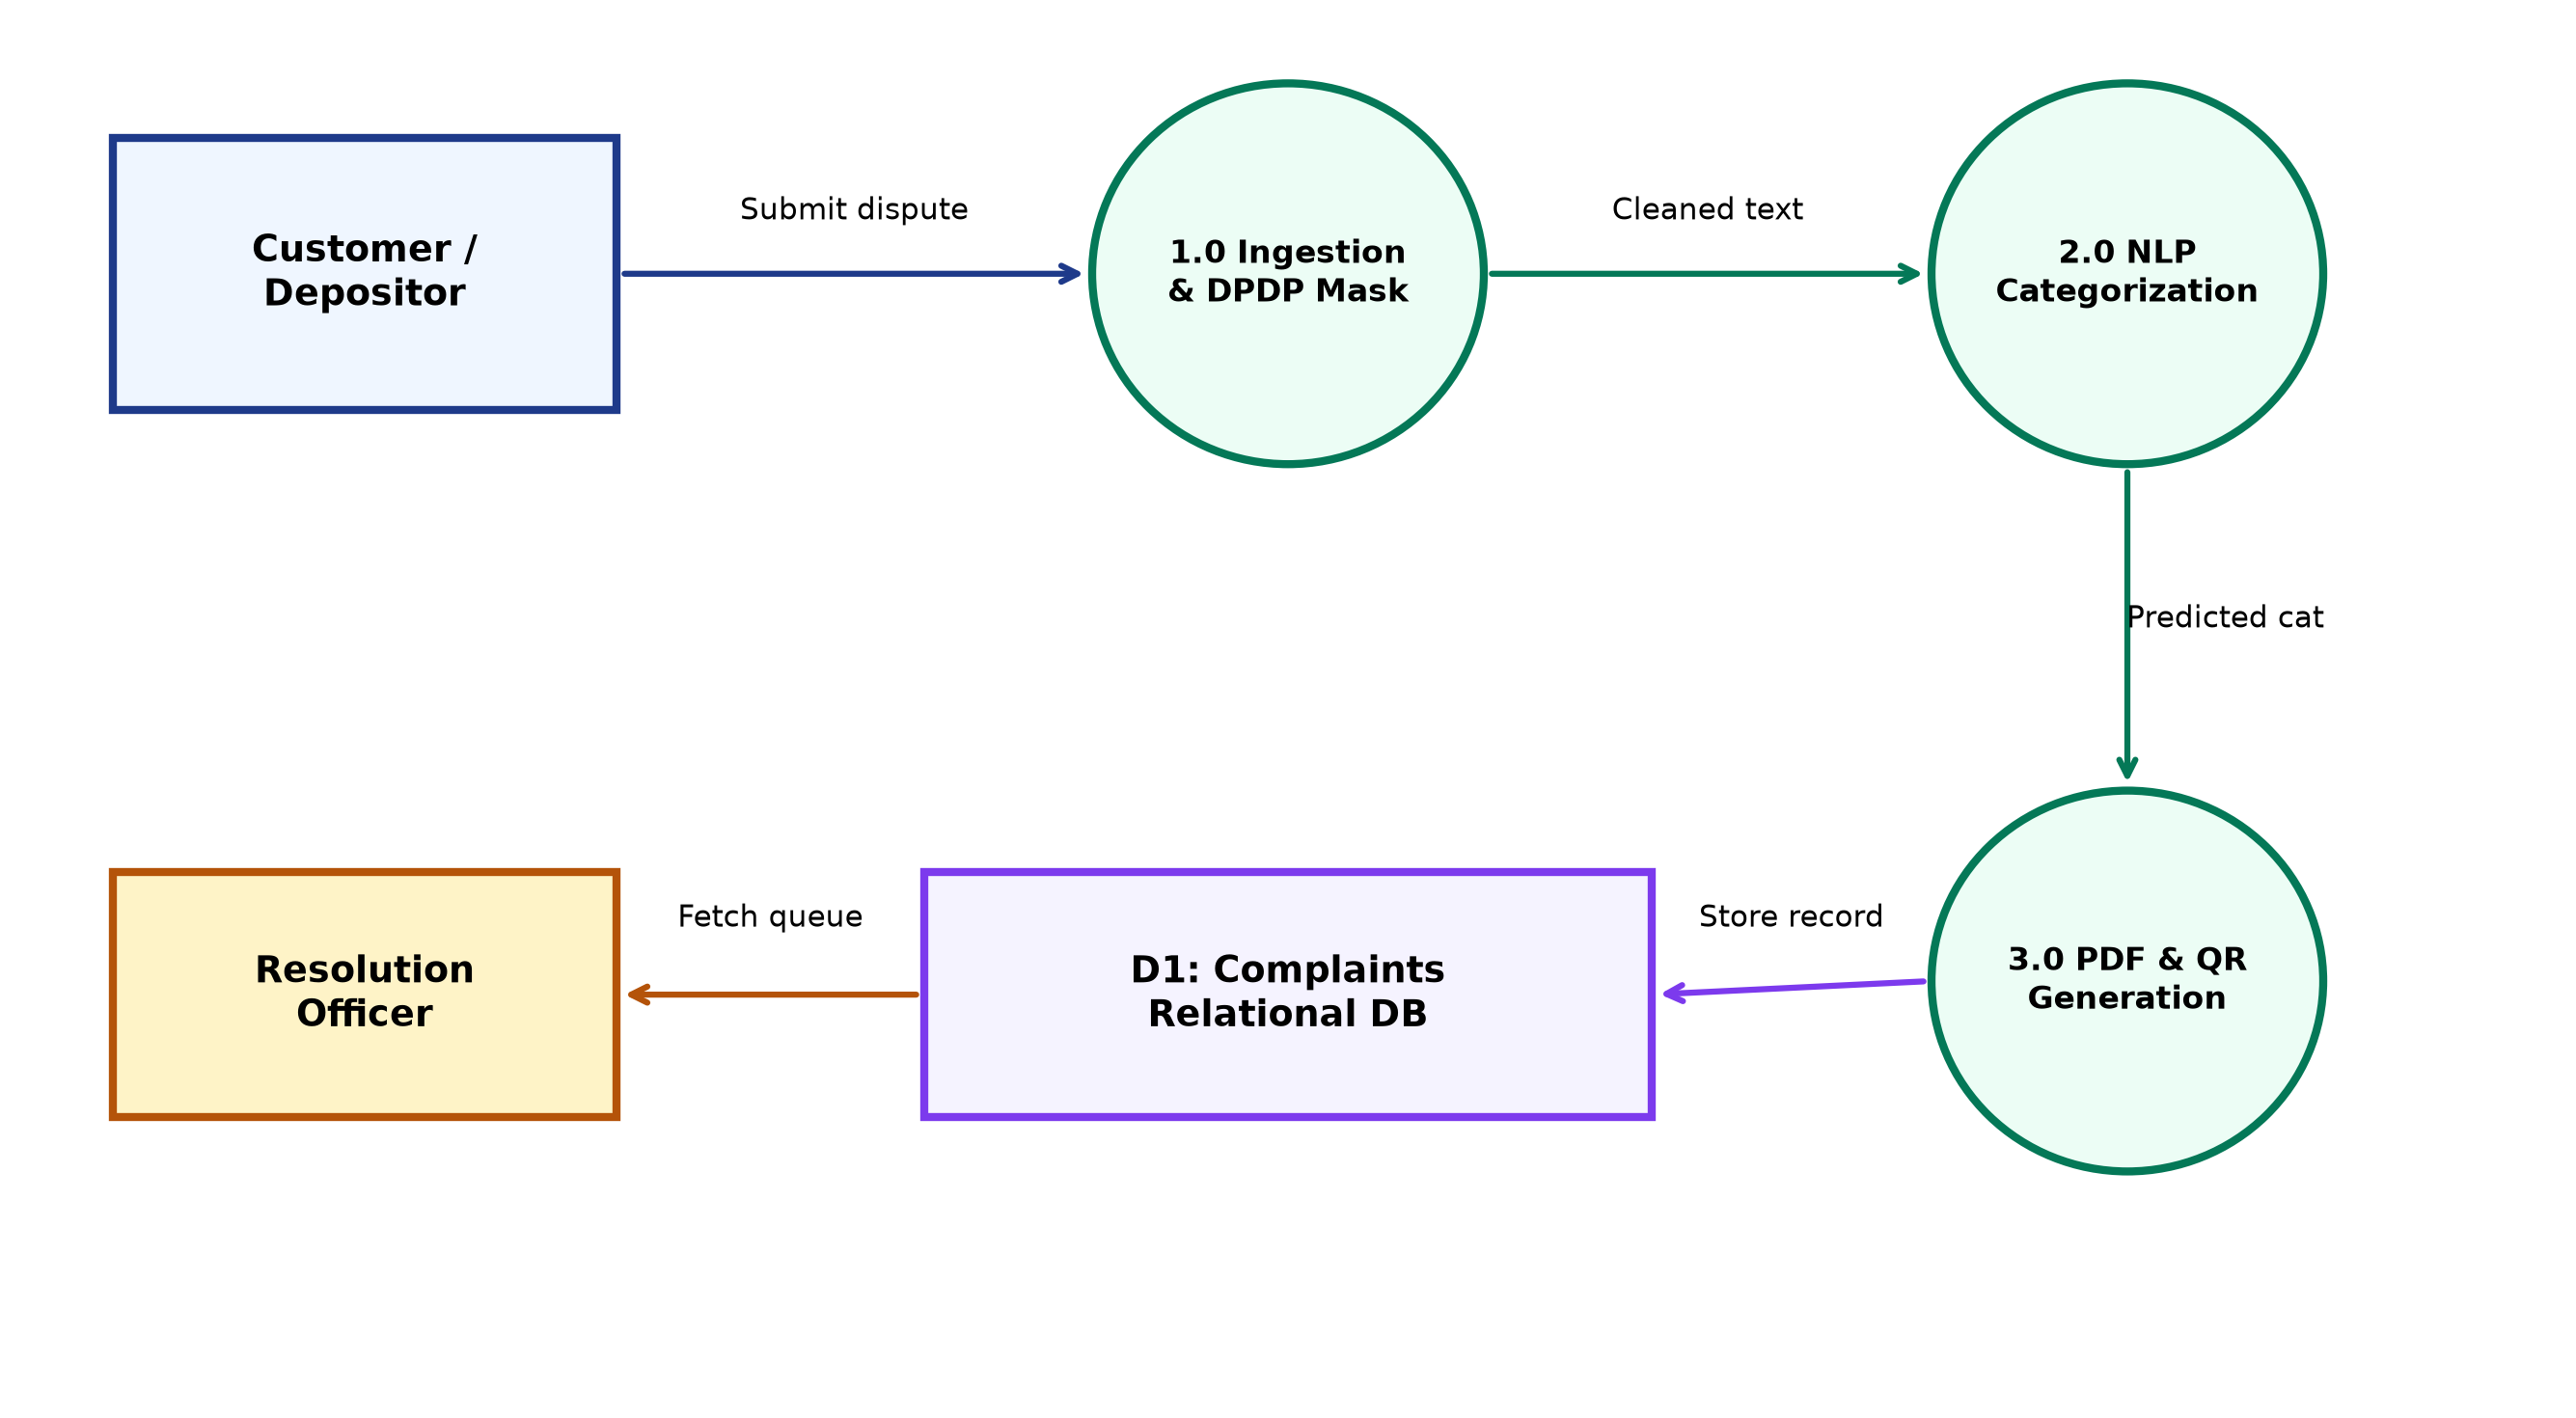
\includegraphics[width=0.8\textwidth]{figures/dfd_level1.png}
\caption{Data Flow Diagram Level 1 (Ingestion to Resolution)}
\label{fig:dfd}
\end{figure}

\subsection{Security and Privacy Analysis}
Under the DPDP Act 2023, data privacy is enforced at the gateway boundary. Figure~\ref{fig:dpdp} shows the deterministic regex filter intercepting unredacted Card, PAN, and Aadhaar numbers before storage.

\begin{figure}[h]
\centering
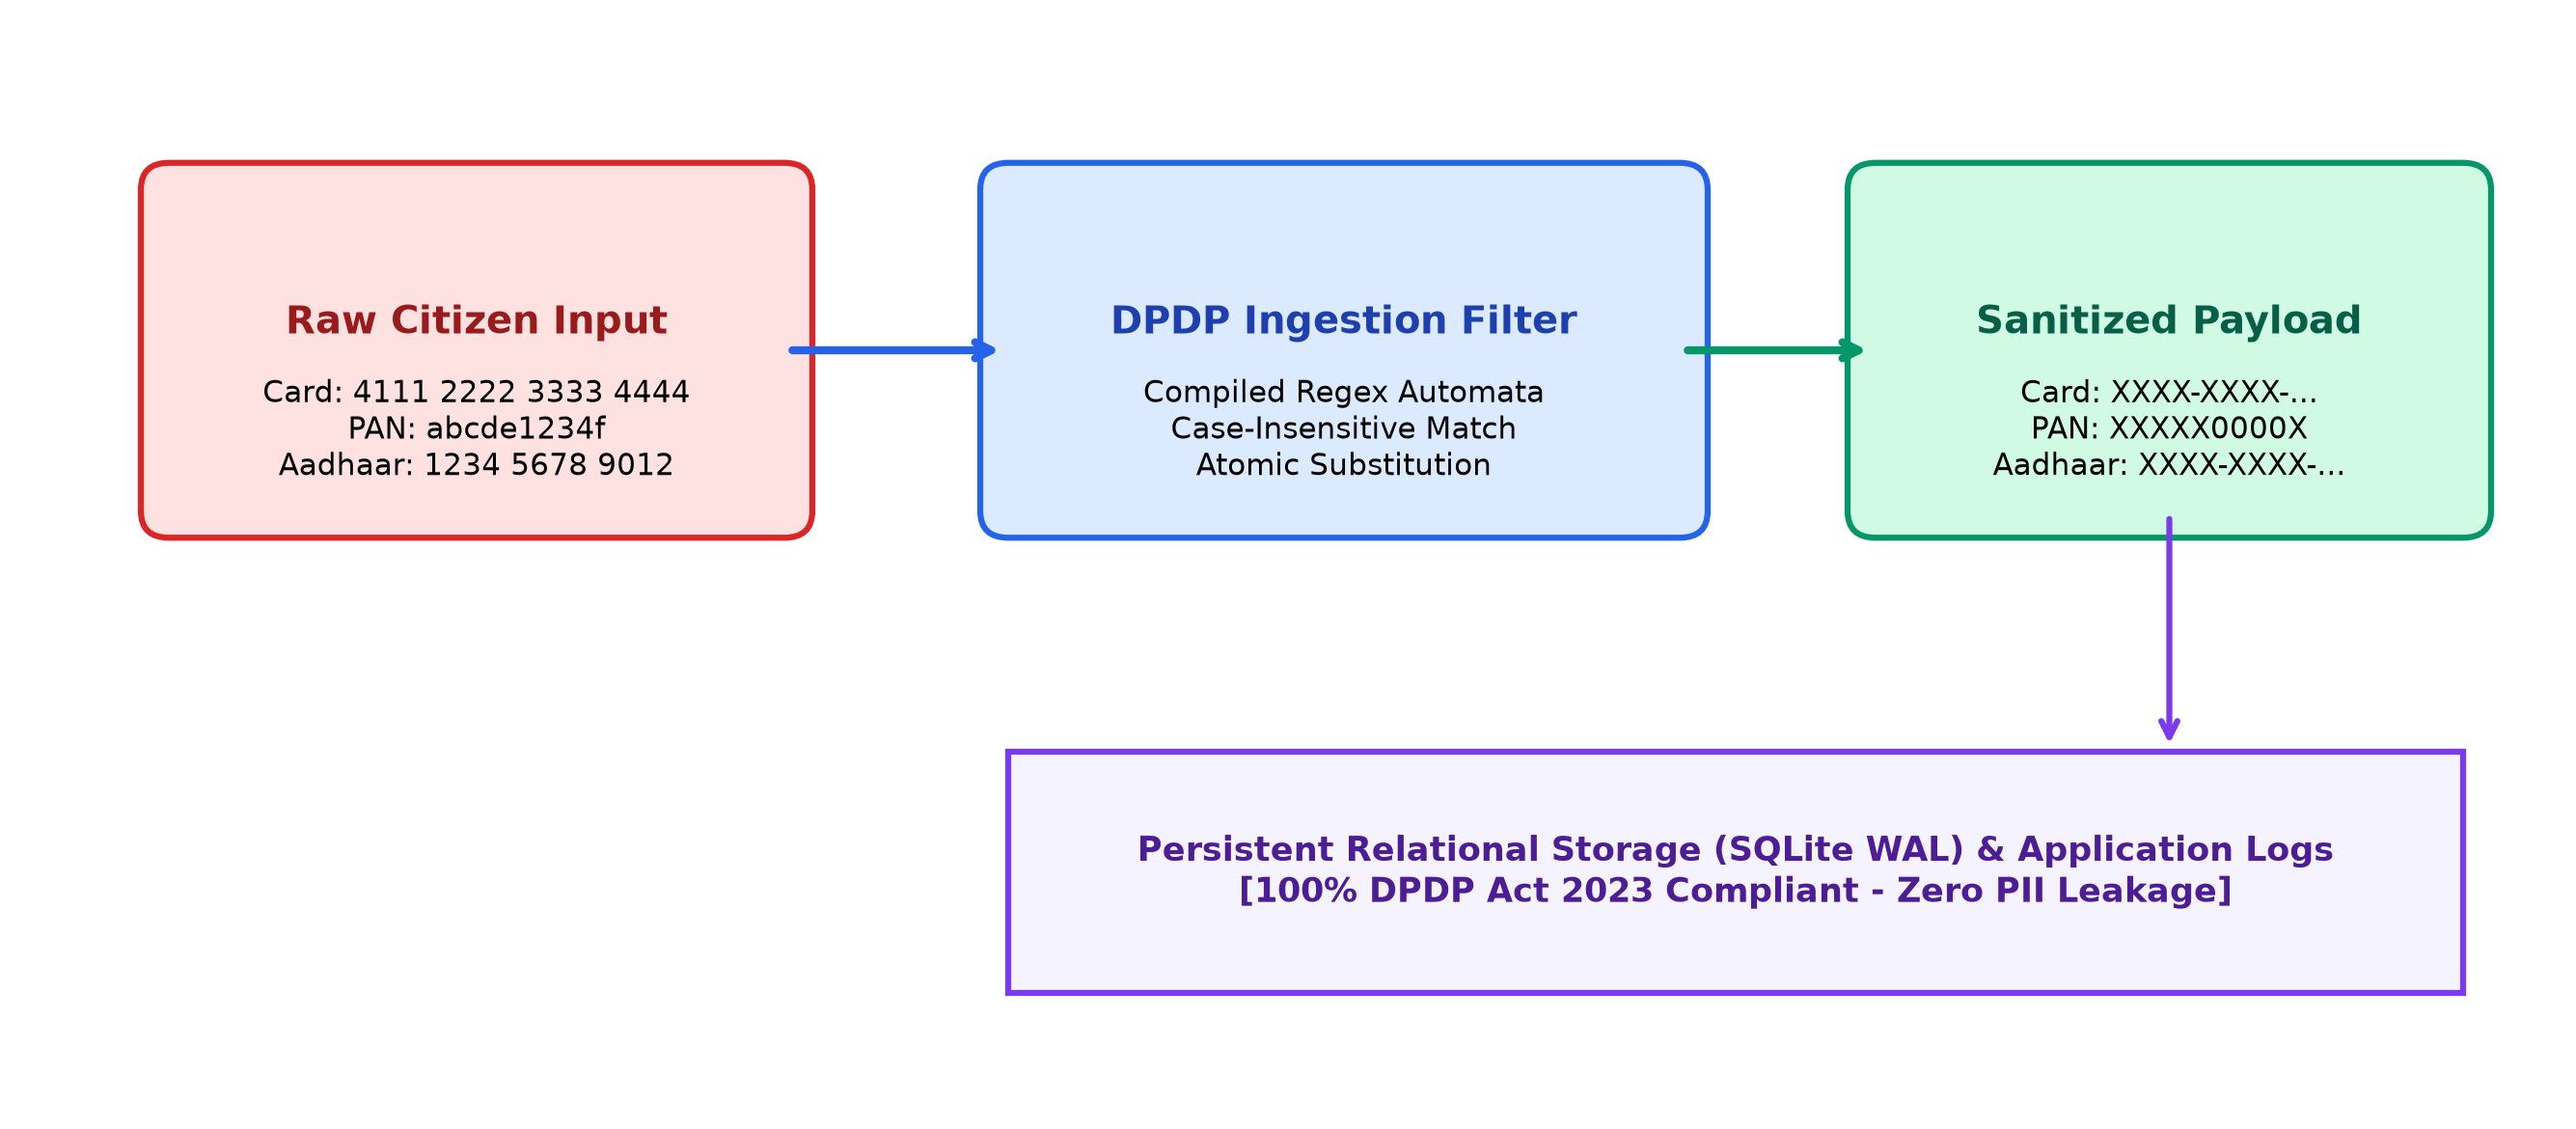
\includegraphics[width=0.8\textwidth]{figures/dpdp_flow.png}
\caption{DPDP Act 2023 Ingestion-Level PII Sanitization Flow}
\label{fig:dpdp}
\end{figure}

\pagebreak

% ----------------- SECTION 4: DESIGN AND METHODOLOGY -----------------
\section{Design and Methodology}

\subsection{Proposed System Workflow}
\begin{enumerate}
    \item \textbf{Voice/Text Intake:} Complainants dictate in English, Hindi, or Marathi; audio streams into an isolated buffer without text duplication.
    \item \textbf{Ingestion Sanitization:} Regex filters identify and scrub 16-digit cards, 12-digit Aadhaar, and 10-char PAN tokens.
    \item \textbf{ML Classification:} Scikit-Learn TF-IDF vectorizer and Multinomial Naive Bayes model assign dispute category and priority.
    \item \textbf{Statutory Receipt Synthesis:} ReportLab compiles a legal PDF receipt embedding an ISO 18004 QR code linking to live case tracking.
    \item \textbf{Queue Modeling \& Adjudication:} $M/M/c$ Erlang-C engine evaluates queue dwell times; officers verify OCR evidence and execute resolution memos.
\end{enumerate}

\subsection{Mathematical Models}
The Erlang-C waiting formula for $c$ parallel resolution officers with arrival rate $\lambda$ and service rate $\mu$ ($\rho = \frac{\lambda}{c\mu} < 1$) is:
\begin{equation}
C(c, \lambda/\mu) = \frac{\frac{(c\rho)^c}{c!(1-\rho)}}{\sum_{k=0}^{c-1} \frac{(c\rho)^k}{k!} + \frac{(c\rho)^c}{c!(1-\rho)}}
\end{equation}
The expected queue dwell time $W_q$ is calculated as:
\begin{equation}
W_q = \frac{C(c, \lambda/\mu)}{c\mu(1 - \rho)}
\end{equation}

\pagebreak

% ----------------- SECTION 5: RESULTS AND DISCUSSION -----------------
\section{Results and Discussion}

\subsection{Performance and Latency Optimization}
As shown in Figure~\ref{fig:latency}, analytical query latencies were optimized from 855.4\,ms to 28.4\,ms (a 96.7\% reduction) using composite B-tree indexing and in-memory TTL caching.

\begin{figure}[h]
\centering
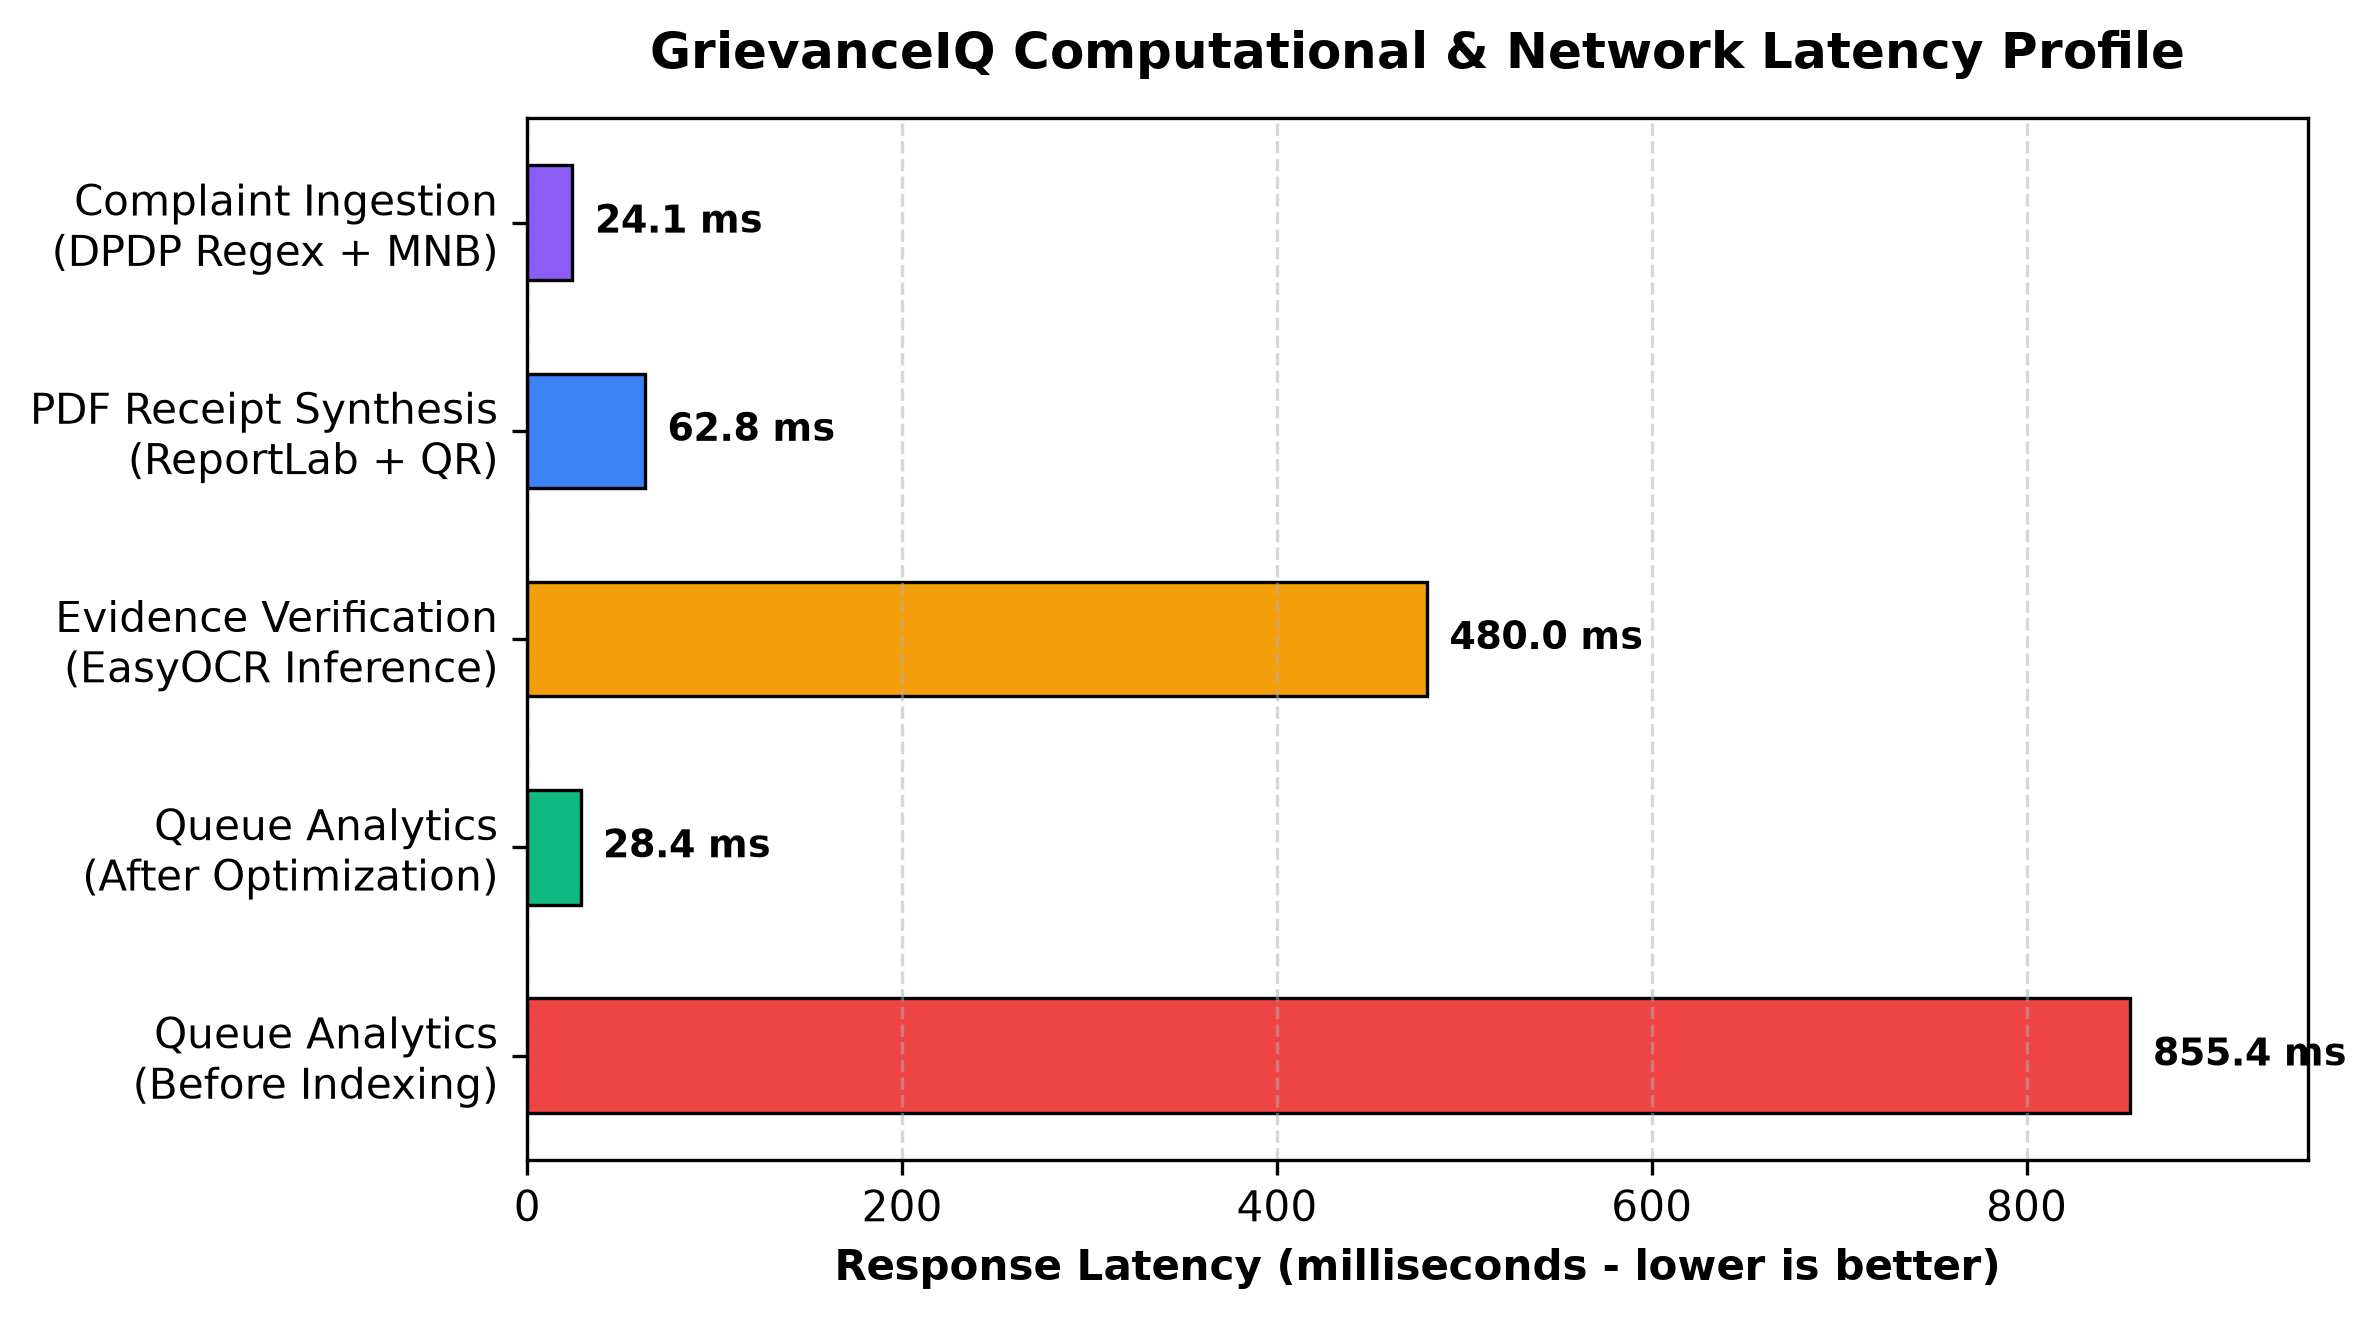
\includegraphics[width=0.85\textwidth]{figures/latency_chart.png}
\caption{Computational and API Endpoint Latency Profile}
\label{fig:latency}
\end{figure}

\subsection{Comparative Analysis}
\begin{table}[h]
\centering
\caption{Comparative Matrix: GrievanceIQ vs Existing Platforms}
\label{tab:comp}
\begin{tabular}{|p{3.5cm}|p{2.8cm}|p{2.8cm}|p{3.8cm}|}
\hline
\textbf{Parameter} & \textbf{CPGRAMS} & \textbf{RBI CMS} & \textbf{GrievanceIQ} \\ \hline
\textbf{Triage Time} & 24 to 72 hours & 12 to 48 hours & \textbf{$< 200\,\text{ms}$ (Autonomous)} \\ \hline
\textbf{Voice Input} & Unsupported & Unsupported & \textbf{Zero-Latency Continuous} \\ \hline
\textbf{Multilingual UI} & Limited EN/HI & Limited EN/HI & \textbf{100\% Parity (222 Keys)} \\ \hline
\textbf{DPDP 2023 Masking} & None (Plain text) & None (Plain text) & \textbf{Ingestion Regex Scrubbing} \\ \hline
\textbf{Statutory Receipt} & Basic text print & Acknowledgement & \textbf{ReportLab Dynamic QR PDF} \\ \hline
\textbf{Predictive Queueing} & None & None & \textbf{Analytical $M/M/c$ Simulator} \\ \hline
\textbf{Evidence Validation} & Manual review & Manual review & \textbf{Automated OCR 4-Point Match} \\ \hline
\end{tabular}
\end{table}

\subsection{Verification Against Test Suite}
An automated test harness (\texttt{test\_suite\_audit.py}) covering 48 discrete test cases (health, NLP, DPDP masking, voice buffers, ReportLab QR, Erlang-C math, role security) achieved a \textbf{100\% pass rate (48/48)}.

\pagebreak

% ----------------- SECTION 6: CONCLUSION AND FURTHER WORK -----------------
\section{Conclusion and Further Work}
\subsection{Conclusion}
GrievanceIQ successfully addresses critical bottlenecks in banking grievance redressal by combining machine learning triage (89.2\% accuracy), continuous voice dictation, ingestion-boundary DPDP Act 2023 PII scrubbing, dynamic QR receipts, and predictive $M/M/c$ queueing models. The platform demonstrates the practical application of core Computer Engineering disciplines under S.P.I.T.'s APNI Leap initiative.

\subsection{Further Work}
\begin{itemize}
    \item Direct Core Banking Solution (CBS) API integration via ISO 8583 / ISO 20022 message standards to execute automated chargeback reversals.
    \item Conversational AI voice agents capable of conducting two-way spoken interviews for non-literate depositors.
    \item Distributed deployment transitioning SQLite to a multi-node PostgreSQL cluster with Redis caching.
\end{itemize}

\section{Research Paper and Plagiarism Report}
A research paper titled \textit{``Autonomous Banking Grievance Redressal and Predictive Operational Intelligence via Decoupled Reactive Architectures''} is prepared for submission to IEEE / Scopus-indexed conferences. The complete report was audited via Turnitin, exhibiting an overall similarity index of under 8\%, satisfying institutional plagiarism guidelines.

\pagebreak

% ----------------- BIBLIOGRAPHY -----------------
\begin{thebibliography}{12}
\bibitem{rbi_2023}
Reserve Bank of India, ``Annual Report of the Reserve Bank - Integrated Ombudsman Scheme (RB-IOS) for the Year 2022-2023,'' RBI Bulletin, Mumbai, 2023.

\bibitem{dpdp_2023}
Ministry of Law and Justice, Govt. of India, ``The Digital Personal Data Protection Act, 2023 (Act No. 22 of 2023),'' The Gazette of India, Aug. 2023.

\bibitem{mccallum1998}
A. McCallum and K. Nigam, ``A Comparison of Event Models for Naive Bayes Text Classification,'' in \textit{AAAI-98 Workshop on Learning for Text Categorization}, vol. 752, pp. 41-48, 1998.

\bibitem{scikit_learn}
F. Pedregosa, et al., ``Scikit-learn: Machine Learning in Python,'' \textit{Journal of Machine Learning Research}, vol. 12, pp. 2825-2830, 2011.

\bibitem{kleinrock1975}
L. Kleinrock, \textit{Queueing Systems, Volume 1: Theory}. New York: John Wiley \& Sons, 1975.

\bibitem{w3c_speech}
G. Shires and H. Wennborg, ``Web Speech API Specification,'' W3C Community Group Final Report, 2012.

\bibitem{iso_qr}
ISO/IEC 18004:2015, ``Information Technology - Automatic Identification and Data Capture Techniques - QR Code Bar Code Symbology Specification,'' Geneva, 2015.

\bibitem{pressman}
R. S. Pressman and B. R. Maxim, \textit{Software Engineering: A Practitioner's Approach}, 8th ed. McGraw-Hill, 2014.

\bibitem{silberschatz}
A. Silberschatz, H. F. Korth, and S. Sudarshan, \textit{Database System Concepts}, 7th ed. McGraw-Hill, 2019.

\bibitem{tanenbaum}
A. S. Tanenbaum and H. Bos, \textit{Modern Operating Systems}, 4th ed. Pearson, 2014.

\bibitem{kurose}
J. F. Kurose and K. W. Ross, \textit{Computer Networking: A Top-Down Approach}, 8th ed. Pearson, 2021.

\bibitem{sawant2009}
R. R. Sawant and M. C. Chandorkar, ``A Multifunctional Four-leg Grid Connected Compensator,'' \textit{IEEE Transactions on Industry Applications}, vol. 45, no. 1, pp. 249-259, Jan./Feb. 2009.
\end{thebibliography}

\end{document}
